\documentclass{article}
\usepackage{amsthm}
\usepackage{amsmath}
\usepackage{graphicx}
\usepackage{multirow}
\usepackage{tikz}
\usepackage{wasysym}
\newtheorem{problem}{Problem}

\begin{document}
\title{Dynamic Programming}
\author{Henry Z. Lo}
\maketitle

\section{Motivating Example}
\subsection{Fibonacci numbers}
\begin{problem}
Given a number $n$, produce the $n^{th}$ Fibonacci number.
\end{problem}

Recall that a Fibonacci number is the sum of the previous two Fibonacci numbers.  The first two Fibonacci numbers are 1:

\[
f(n) = \begin{cases} 
1 &\mbox{if } n=1 \mbox{ or } n=2 \\ 
f(n-2)+f(n-1) & \mbox{otherwise }
\end{cases} 
\]

\subsubsection{Brute force solution}
The obvious algorithm would be to follow this recursive formula, yielding the computation tree seen in Figure \ref{fibonacci}.  For each number from 1 to $n$, the algorithm spawns off two recursive calls - thus, time complexity is $O(2^n)$.

\begin{figure}
\centering
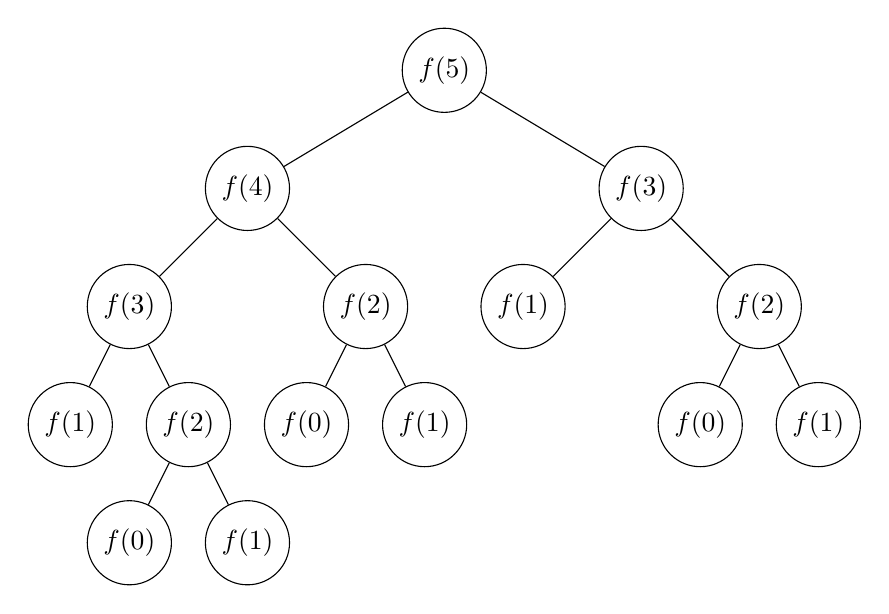
\begin{tikzpicture}[level 1/.style={sibling distance=50mm},
level 2/.style={sibling distance=30mm},
level 3/.style={sibling distance=15mm}]
\tikzstyle{every node}=[circle,draw]
\node {$f(5)$}
child{ node {$f(4)$}
	child{ node {$f(3)$}
		child{ node {$f(1)$}}
		child{ node {$f(2)$}
			child{ node {$f(0)$}}
			child{ node {$f(1)$}}
		}
	}
	child{ node {$f(2)$}
		child{ node {$f(0)$}}
		child{ node {$f(1)$}}
	}
}
child{ node {$f(3)$}
		child{ node {$f(1)$}}
		child{ node {$f(2)$}
			child{ node {$f(0)$}}
			child{ node {$f(1)$}}
		}
	}
;
\end{tikzpicture}
\caption{Computation tree for calculating the 5th Fibonacci number.\label{fibonacci}}
\end{figure}

\subsubsection{Memoization}
Note in the computation of this algorithm, there are \textit{overlapping subproblems} - for example, $f(2)$ is computed 3 times, and $f(3)$ is computed twice.  We can save entire subtrees if we simply store (memoize) the result of $f(2)$ and $f(3)$, and then simply try a lookup next time $f(2)$ or $f(3)$ is needed.  

See Figure \ref{fibonacci-memo} for a visual.

\begin{figure}
\centering
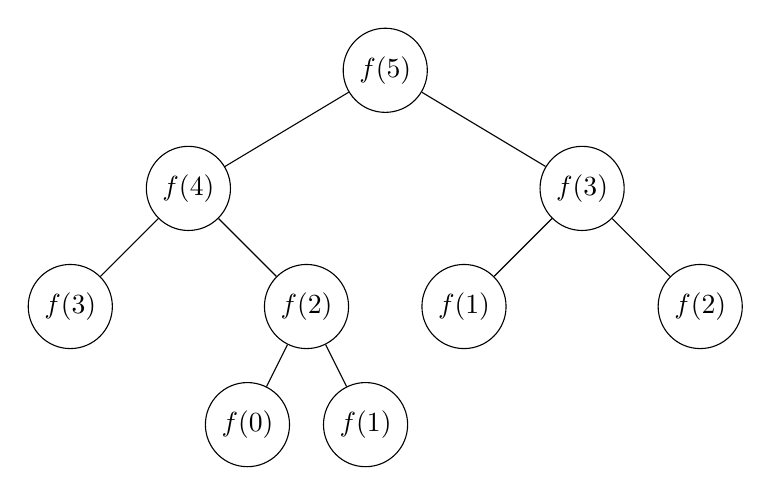
\begin{tikzpicture}[level 1/.style={sibling distance=50mm},
level 2/.style={sibling distance=30mm},
level 3/.style={sibling distance=15mm}]
\tikzstyle{every node}=[circle,draw]
\node {$f(5)$}
child{ node {$f(4)$}
	child{ node {$f(3)$}}
	child{ node {$f(2)$}
		child{ node {$f(0)$}}
		child{ node {$f(1)$}}
	}
}
child{ node {$f(3)$}
		child{ node {$f(1)$}}
		child{ node {$f(2)$}}
	}
;
\end{tikzpicture}
\caption{Fibonacci computation tree, with memoization.\label{fibonacci-memo}}
\end{figure}

\begin{figure}
\centering
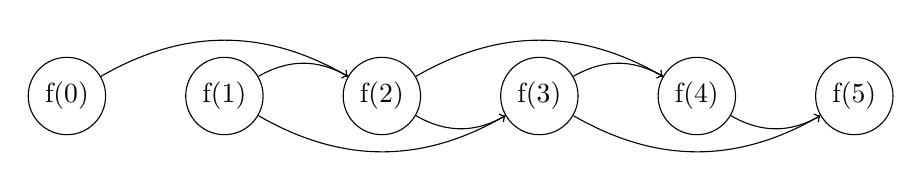
\begin{tikzpicture}[->,node distance=2cm, main node/.style={draw,circle}]
\node[main node] (0){f(0)};
\node[main node, right of=0](1){f(1)};
\node[main node, right of=1](2){f(2)};
\node[main node, right of=2](3){f(3)};
\node[main node, right of=3](4){f(4)};
\node[main node, right of=4](5){f(5)};

\path
(0) [bend left] edge node {} (2)
(1) edge node {} (2)
(1) [bend right] edge node {} (3)
(2) edge node {} (3)
(2) [bend left] edge node {} (4)
(3) edge node {} (4)
(3) [bend right] edge node {} (5)
(4) edge node {} (5);
\end{tikzpicture}
\caption{Fibonacci computations, with dynamic programming.\label{fibonacci-dynamic}}
\end{figure}

How fast is this new algorithm?  Well, notice that each Fibonacci number is only calculated once.  Thus, this algorithm requires roughly $O(n)$ computations.

\subsubsection{Dynamic programming approach}
Another method to avoid computing Fibonacci numbers repeatedly is to compute them from the bottom up.  For this problem, we can simply compute the Fibonacci numbers up from 2 to $n$ (see Figure \ref{coin_dp}).

$f(2)$ only involves one computation, and once we have $f(2)$, $f(3)$ can be calculated in one step.  Thus, continuing up to $n$ requires $O(n)$ computations.

\section{Dynamic Programming}
\subsection{Change making revisited}
\begin{problem}
Given a value $n$, and a set of coins $c_1,...,c_m$, find the minimal set of coins summing up to $n$.
\end{problem}

Though the greedy method worked for the U.S. and probably most modern currencies, it does not work in general for all coinages.  Let's consider a currency with $1\cent, 4\cent, 5\cent$, and a value of $12\cent$.

We use this example to demonstrate dynamic programming, which can get the correct answer.

\begin{figure}
\centering
\resizebox{1\linewidth}{!}{
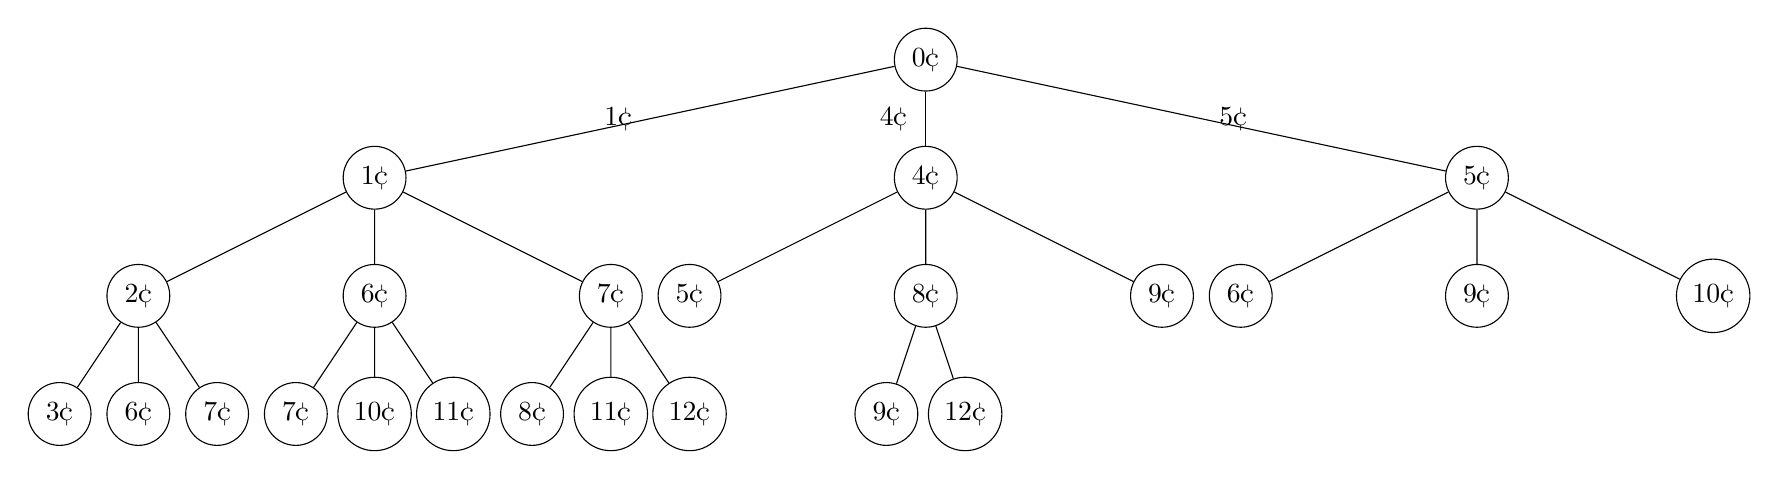
\begin{tikzpicture}[level 1/.style={sibling distance=70mm},
level 2/.style={sibling distance=30mm},
level 3/.style={sibling distance=10mm}]
\tikzstyle{every node}=[circle,draw]

\node {$0\cent$}
child{ node {$1\cent$} 
	child{ node {$2\cent$} 
		child{ node {$3\cent$}}
		child{ node {$6\cent$}}
		child{ node {$7\cent$}}
	}
	child{ node {$6\cent$}
		child{ node {$7\cent$}}
		child{ node {$10\cent$}}
		child{ node {$11\cent$}}
	}
	child{ node {$7\cent$}
		child{ node {$8\cent$}}
		child{ node {$11\cent$}}
		child{ node {$12\cent$}}
	}
edge from parent node[left,draw=none] {$1\cent$}
}
child{ node {$4\cent$} 
	child{ node {$5\cent$}}
	child{ node {$8\cent$} 
		child{ node {$9\cent$}}
		child{ node {$12\cent$}}
	}
	child{ node {$9\cent$}}
edge from parent node[left,draw=none] {$4\cent$}
}
child{ node {$5\cent$} 
	child{ node {$6\cent$}}
	child{ node {$9\cent$}}
	child{ node {$10\cent$}}
edge from parent node[right,draw=none] {$5\cent$}
}
;
\end{tikzpicture}}
\caption{Bottom-up computation tree for the change-making problem.\label{coin_dp}}
\end{figure}

\subsection{Brute force search}
Dynamic programming works on programs where you need to calculate every possible option sequentially.  This leads to computation paths which can be modeled in a tree.  Finding a solution is equivalent to performing a breadth-first search in this tree.

For example, the computation tree in Figure \ref{fibonacci} shows every computation path that can be taken.  For the change making program, Figure \ref{coin_dp} shows a partial computation tree -- it would be complete if we expand all $7\cent$ and $6\cent$ nodes.

Where the same value appears in multiple nodes in the tree, this means that multiple computation paths lead to the same computation state, i.e. there are \textit{overlapping subproblems}.  In Figure \ref{coin_dp}, there are three ways to get to $7\cent$: using $1\cent$ and $4\cent$, $4\cent$ then $1\cent$, or $5\cent$.  But how we got to $7\cent$ has no bearing on how we select coins in the future, so we should only regard the optimal path to $7\cent$, which is $5\cent$.

\subsection{Problems which can be solved}

In other words, when we have overlapping subproblems, we can disregard those paths which are not optimal.

Thus, dynamic programming requires two properties of problems:
\begin{itemize}
\item \textbf{Optimal substructure}: An optimal solution can be computed from optimal solutions of its subproblems.  This allows us to keep paths that are optimal, because they will be useful for calculating the final solution.
\item \textbf{Overlapping subproblems}: This property states that the problem can be broken down into smaller problems, and many of these smaller problems are the same.  This allows us to save computations by storing results.
\end{itemize}

We have already seen optimal substructure.  Overlapping subproblems is needed because otherwise, there would be no point in remembering the subproblem answers (as in our change-making example).  The optimal substructure property guarantees that the solutions to our subproblems are still useful.

Intuitively, a problem can be improved by dynamic programming if its computation tree actually forms a graph (same nodes appear at multiple places in the tree).

\subsection{Memoization}
One simple way to memorize previous results is to perform the computation top-down.  As we solve subproblems, we \textit{memoize} their solutions, so that they do not need to be computed when we encounter them again.

Figure \ref{fibonacci-memo} shows the bottom-up memoization approach for the Fibonacci problem, and Figure \ref{coin_tree} for the coin problem.

\begin{figure}
\centering
\resizebox{1\linewidth}{!}{
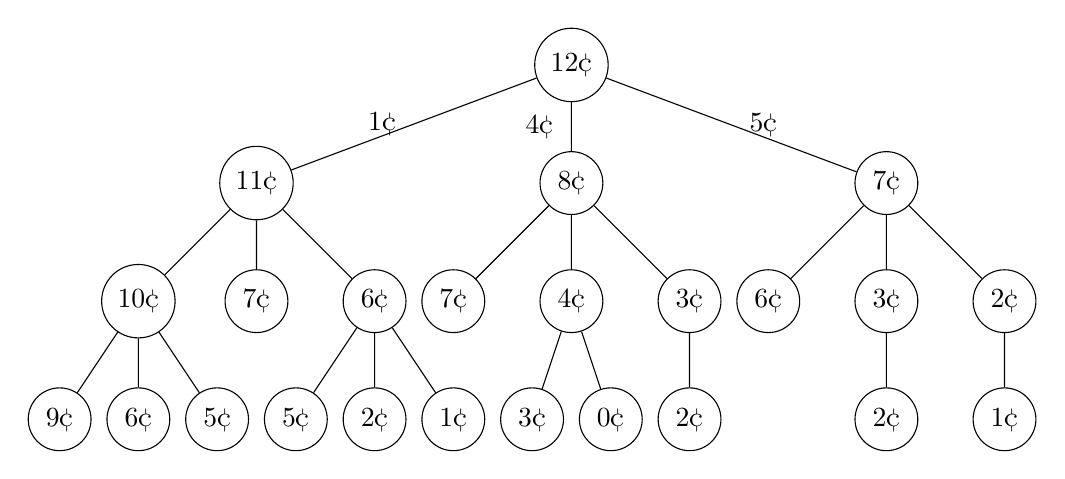
\begin{tikzpicture}[level 1/.style={sibling distance=40mm},
level 2/.style={sibling distance=15mm},
level 3/.style={sibling distance=10mm}]
\tikzstyle{every node}=[circle,draw]

\node {$12\cent$}
child{ node {$11\cent$} 
	child{ node {$10\cent$} 
		child{ node {$9\cent$}}
		child{ node {$6\cent$}}
		child{ node {$5\cent$}}
	}
	child{ node {$7\cent$}}
	child{ node {$6\cent$}
		child{ node {$5\cent$}}
		child{ node {$2\cent$}}
		child{ node {$1\cent$}}
	}
edge from parent node[left,draw=none] {$1\cent$}
}
child{ node {$8\cent$} 
	child{ node {$7\cent$}}
	child{ node {$4\cent$} 
		child{ node {$3\cent$}}
		child{ node {$0\cent$}}
	}
	child{ node {$3\cent$}
		child{ node {$2\cent$}}
	}
edge from parent node[left,draw=none] {$4\cent$}
}
child{ node {$7\cent$} 
	child{ node {$6\cent$}}
	child{ node {$3\cent$} 
		child{ node {$2\cent$}}
	}
	child{ node {$2\cent$}
		child{ node {$1\cent$}}
	}
edge from parent node[right,draw=none] {$5\cent$}
}
;
\end{tikzpicture}}
\caption{Top-down computation tree for the change-making problem.\label{coin_tree}}
\end{figure}

In this approach, we only solve subproblems as needed.  When we do solve it, we cache the solution (store it in a hashmap or something).  In practice, this is easier to code, since we solve the problems exactly as before.

\subsection{Dynamic programming}
Technically, \textit{memoization} is a type of dynamic programming, but dynamic programming usually refers to the bottom-up approach.  This is exemplified in Figures \ref{fibonacci-dynamic} and \ref{coin_dp}.

This approach computes smaller solutions in the hopes that they will be useful for reaching the larger solutions.  This is typically harder to program, because the memorization is implicit in the algorithm.

\section{Examples}
\subsection{Maximum contiguous subarray}
\begin{problem}
Given an integer array, find the subarray with the largest sum.  The subarray must be contiguous, i.e. it must contain every element between its start and end.
\end{problem}

For example, for the array \texttt{[-9,4,6,-7,3]}, the solution is \texttt{[4,6]}.  The computation tree for this array is:

\begin{figure}
\centering
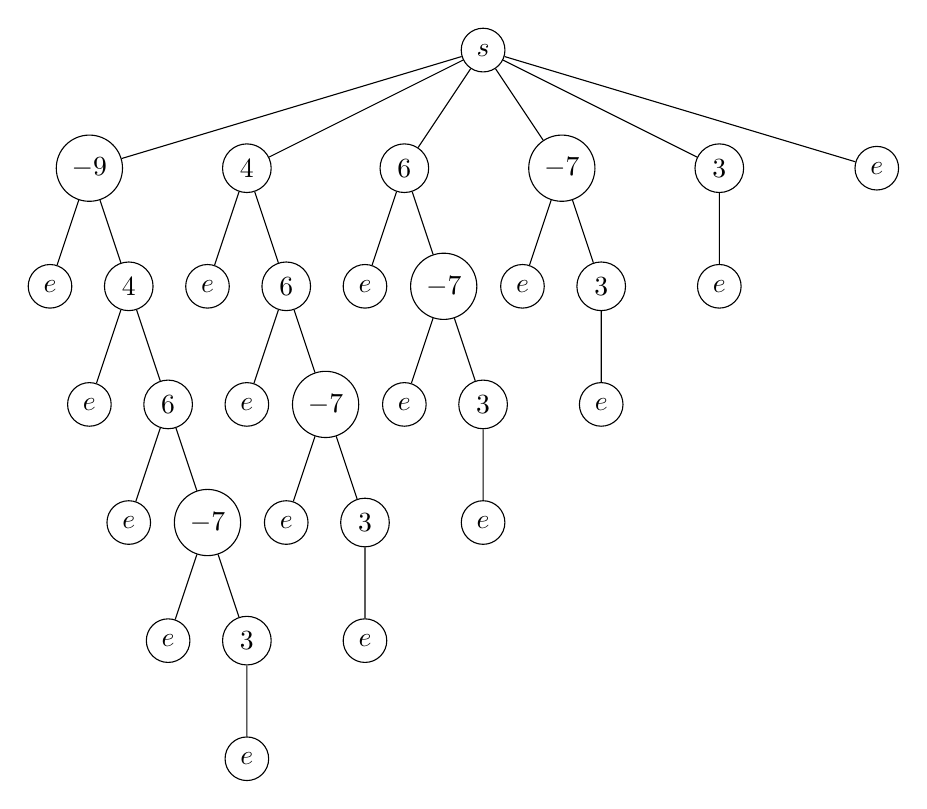
\begin{tikzpicture}[level 1/.style={sibling distance=20mm},
level 2/.style={sibling distance=10mm}]
\tikzstyle{every node}=[circle,draw]

\node {$s$}
child{ node {$-9$}
	child{ node {$e$}}
	child{ node {$4$}
		child{ node {$e$}}
		child{ node {$6$}
			child{ node {$e$}}
			child{ node {$-7$}
				child{ node {$e$}}
				child{ node {$3$}
					child{ node {$e$}}
				}
			}
		}
	}
}
child{ node {$4$}
	child{ node {$e$}}
	child{ node {$6$}
		child{ node {$e$}}
		child{ node {$-7$}
			child{ node {$e$}}
			child{ node {$3$}
				child{ node {$e$}}
			}
		}
	}
}
child{ node {$6$}
	child{ node {$e$}}
	child{ node {$-7$}
		child{ node {$e$}}
		child{ node {$3$}
			child{ node {$e$}}
		}
	}
}
child{ node {$-7$}
	child{ node {$e$}}
	child{ node {$3$}
		child{ node {$e$}}
	}
}
child{ node {$3$}
	child{ node {$e$}}
}
child{ node {$e$}}
;
\end{tikzpicture}
\caption{Computation tree for the maximum subarray problem.  $s$ stands for start, and $e$ stands for end.  \label{array_tree}}
\end{figure}

In this problem, we must search the whole tree, because we do not have a fixed target to reach.  We just want to maximize the sum along the path.

Note that there are many many overlapping problems here.  Thus, we can reduce the problem to the graph in Figure \ref{array_graph}.

\begin{figure}
\centering
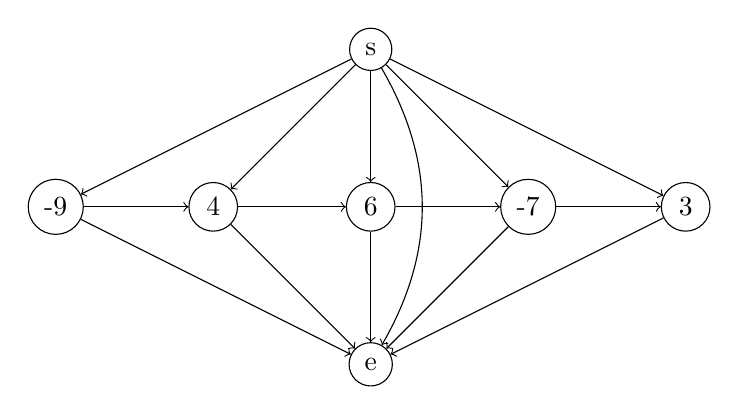
\begin{tikzpicture}[->,node distance=2cm, main node/.style={draw,circle}]
\node[main node] (s){s};
\node[main node, below of=s] (6) {6};
\node[main node, left of=6]  (4) {4};
\node[main node, right of=6](-7){-7};
\node[main node, left of=4]  (-9){-9};
\node[main node, right of=-7] (3) {3};
\node[main node, below of=6] (e) {e};

\path
(s) edge node {} (-9)
    edge node {} (4)
    edge node {} (6)
    edge node {} (-7)
    edge node {} (3)
(-9)edge node {} (4)
    edge node {} (e)
(4) edge node {} (6)
    edge node {} (e)
(6)edge node {} (-7)
    edge node {} (e)
(-7)edge node {} (3)
    edge node {} (e)
(3) edge node {} (e)
(s) [bend left] edge node {} (e)
;
\end{tikzpicture}
\caption{Reduced graph for the maximum subarray problem.\label{array_graph}}
\end{figure}

Along with this reduced computation graph, we can take advantage of the following facts:
\begin{itemize}
\item If our current path sum is 0, we can discard the entire path, since the empty path is better.
\item If our current path is positive, and
\begin{itemize}
\item if the node to the right is positive, we move to it, since we can increase the current path sum.
\item otherwise, we end the path, and record it.
\end{itemize}
\item If we have already visited a node from the left, we can disregard it; this is because it has already been considered in a larger sum path.
\end{itemize}

Putting these facts together, we can come up with an $O(n)$ algorithm which traverses the list only once.

\subsubsection{Algorithm}
For simplicity, we return the sum over the maximum sequence.  By simple extension we can return the start and the end of the maximum sequence instead.

\begin{verbatim}
max_subarray(a) {
  sum = 0
  max_sum = 0
  // i here is the number, not the index
  for (i in a)  {
    if (i > 0) {
      sum += i
    } else {
      max_sum = sum
      // if negative is larger than sum, then not worth it
      if ((sum + i) < 0) {
        sum = 0
      }
    }
  }
  return(max(sum, max_sum))
}
\end{verbatim}

\subsection{Edit distance}

\begin{problem}
There are two strings, $x$ and $y$.  We want to calculate the edit distance between them.  Edit distance is the minimal amount of insertions, deletions, and edits to morph one string into the other. 
\end{problem}

This problem is often encountered in comparing DNA sequences.

As an example, the edit distance between \texttt{at} and \texttt{sit} is 2.
\[
\texttt{at} \rightarrow \texttt{sat} \rightarrow \texttt{sit}
\]

We have to be careful about how we define the computation tree, otherwise it can be enormous.  Note that to properly calculate edit distance, we need to:
\begin{itemize}
\item Compare characters in $x$ with characters in $y$.
\item Start this comparison from the beginning of both $x$ and $y$.
\item Finish at the end of $x$, $y$, or both.
\end{itemize}
Thus, we define each node to be a comparison of a character in $x$ and a character in $y$.  Thus, we start at $s\texttt{-}s$,, and move up either one character in $x$ (addition), one character in $y$ (deletion), or both (matching), until we get to the end of one string.

The partial computation tree (with repeated subtrees not computed) is shown in Figure \ref{edit_tree}.  The goal is to maximize matches, and minimize every other type of node.

\begin{figure}
\centering
\resizebox{1\linewidth}{!}{
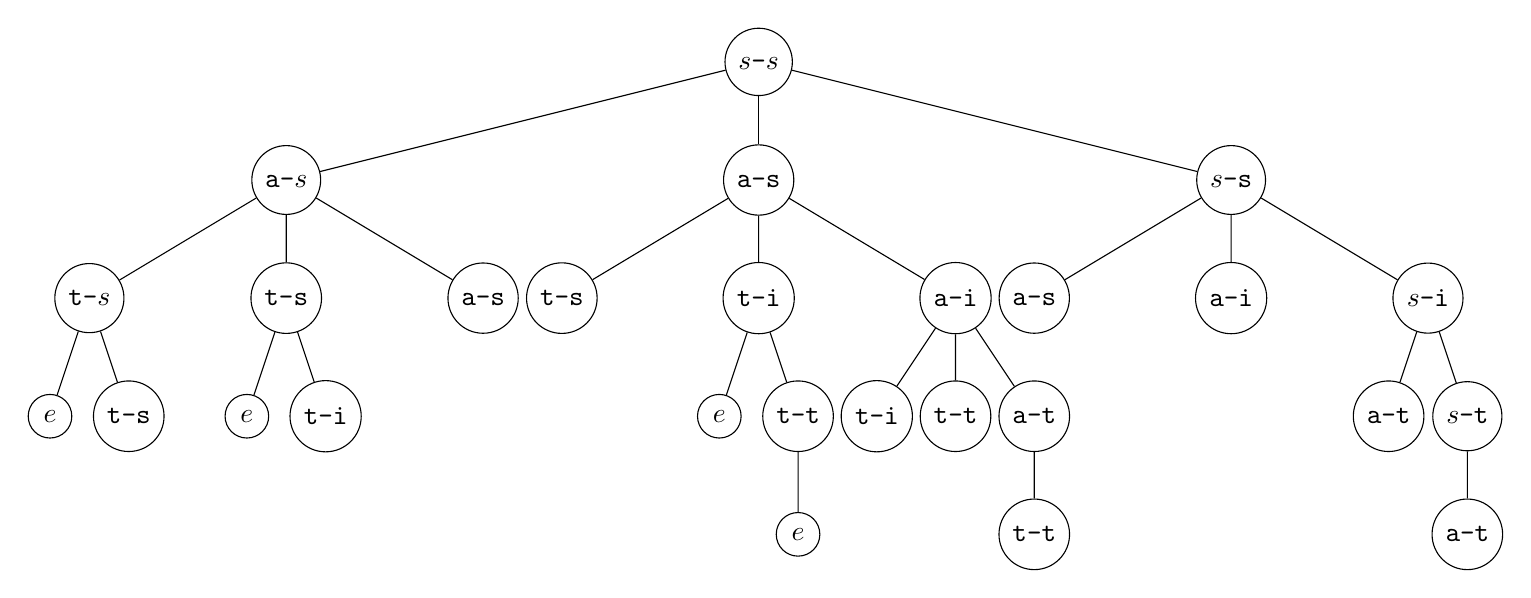
\begin{tikzpicture}[level 1/.style={sibling distance=60mm},
level 2/.style={sibling distance=25mm},
level 3/.style={sibling distance=10mm},]
\tikzstyle{every node}=[circle,draw]

\node {$s\texttt{-}s$}
child{ node {$\texttt{a-}s$}
	child{ node {$\texttt{t-}s$}
		child{ node {$e$}}
		child{ node {$\texttt{t-s}$}}
	}
	child{ node {$\texttt{t-s}$}
		child{ node {$e$}}
		child{ node {$\texttt{t-i}$}}
	}
	child{ node {$\texttt{a-s}$}}
}
child{ node {$\texttt{a-s}$}
	child{ node {$\texttt{t-s}$}}
	child{ node {$\texttt{t-i}$}
		child{ node {$e$}}	
		child{ node {$\texttt{t-t}$}
			child{ node {$e$}}
		}
	}
	child{ node {$\texttt{a-i}$}
		child{ node {$\texttt{t-i}$}}
		child{ node {$\texttt{t-t}$}}
		child{ node {$\texttt{a-t}$}
			child{ node {$\texttt{t-t}$}
			}
		}
	}
}
child{ node {$s\texttt{-s}$}
	child{ node {$\texttt{a-s}$}}
	child{ node {$\texttt{a-i}$}}
	child{ node {$s\texttt{-i}$}
		child{ node {$\texttt{a-t}$}}
		child{ node {$s\texttt{-t}$}
			child{ node {$\texttt{a-t}$}}
		}
	}
}
;
\end{tikzpicture}}
\caption{Partial computation tree for the edit distance problem, for strings \texttt{at} and \texttt{sit}.  $s$ stands for start, $e$ represents the end of matching.  \label{edit_tree}}
\end{figure}

The Wagner-Fischer algorithm notes that this type of tree can actually be represented using a matrix, as seen in Figure \ref{edit_matrix}:
\begin{itemize}
\item Top left represents root.
\item Edges represent leaves.
\item From each square, we can move below (insert), to the right (delete), or bottom right (match).
\item The values in the square represent the cumulative distance of the path.
\item The goal is to find the path from the top left to an edge with the minimum distance.
\item Each node's value is the minimum of its predecessors' values, plus one if it's not a match.
\end{itemize} 

\begin{table}
\centering
\begin{tabular}{c|ccc}
 & &\texttt{a} &\texttt{t} \\
\hline
  & 0 & 1 & 2 \\
\texttt{s} & 1 & 1 & 2 \\
\texttt{i} & 2 & 2 & 2 \\
\texttt{t} & 3 & 3 & 2
\end{tabular}
\caption{Matrix generated by the Wagner-Fischer algorithm for computing edit distance \label{edit_matrix}}
\end{table}

The last fact takes advantage of the optimal substructure of the problem.  By condensing the overlapping problems in the computation tree into a matrix form, we reduce computation time to $O(mn)$, where $m$ and $n$ are the lengths of the two strings.

\end{document}
